\documentclass[12pt, a4paper]{article}
\usepackage{graphicx} % Required for inserting images
\usepackage{float}  % para poner imagen en lugar
\usepackage{subfigure} % para poner varios imagenes en el lugar
\usepackage[width=150mm, bottom=3cm, top=3cm]{geometry} % ajustar margenes del doc
\usepackage{comment} % Para hacer comentarios largos
\usepackage{caption} % Para ajustar la descripcion de las imagenes
\usepackage{amsfonts, amsmath, amssymb}
\usepackage{tcolorbox} % Para colores
\tcbuselibrary{minted,breakable,xparse,skins}
\usepackage{hyperref}
\usepackage[english, spanish]{babel}

% Configuracion de código en Python
\DeclareTCBListing{mintedbox}{O{}m!O{}}{%
  breakable=true,
  listing engine=minted,
  listing only,
  minted language=#2,
  minted style=default,
  minted options={%
    linenos,
    gobble=0,
    breaklines=true,
    breakafter=,,
    fontsize=\small,
    numbersep=8pt,
    #1},
  boxsep=0pt,
  left skip=0pt,
  right skip=0pt,
  left=25pt,
  right=0pt,
  top=3pt,
  bottom=3pt,
  arc=5pt,
  leftrule=0pt,
  rightrule=0pt,
  bottomrule=2pt,
  toprule=2pt,
  colback=bg,
  colframe=orange!70,
  enhanced,
  overlay={%
    \begin{tcbclipinterior}
    \fill[orange!20!white] (frame.south west) rectangle ([xshift=20pt]frame.north west);
    \end{tcbclipinterior}},
  #3}


% Títulos 
\title{Análisis de Simulaciones\\[3pt] Física sexto año CNBA}
\vspace{3cm}
\author{Ian Chen, Lola Cavalieri, Matías Flory, Ana Barrientos}
\date{Julio 2024}


%%%%%%%%%%%%%%%%%%%%%%%%%%%%%%%
\begin{document}

\maketitle

\vspace{10pt}
\selectlanguage{spanish}
\begin{abstract}
El siguiente trabajo presenta un análisis detallado y una comparación de diversas simulaciones computacionales de movimientos físicos, centrándose específicamente en tres tipos fundamentales: el movimiento recto, el movimiento circular y las ondas. Este estudio se lleva a cabo utilizando Simple GUI en Python 2.7, que permite una interacción intuitiva y visualización clara de los conceptos físicos involucrados. 
\end{abstract}

\selectlanguage{english}
\begin{abstract}
The following work presents a detailed analysis and a comprehensive comparison of various computational simulations of physical movements, focusing specifically on three fundamental types: rectilinear motion, circular motion, and waves. This study is carried out using Simple GUI in Python 2.7, which allows for intuitive interaction and clear visualization of the physical concepts involved.
\end{abstract}


%%%%%%%%%%%%%%%%%%%%%%%%%%%%%%%
\newpage
\selectlanguage{spanish}
\section{Introduction}
Este trabajo se centra en la creación y comparación de diversas simulaciones de movimientos físicos. Empleando Simple GUI en Python 2.7, se han desarrollado simulaciones que permiten una visualización clara de los fenómenos simulados. El objetivo principal es evaluar la eficacia de estas simulaciones en la replicación de comportamientos físicos y su potencial como herramientas de predicción.


\section{Primera Parte - Movimiento circular}
Para esta primera parte del trabajo se van a realizar las simulaciones utilizando el código que se encuentra en el archivo movimiento\_v2.txt dado por el docente del curso. En este caso se trata de un movimiento circular. 


Para el estudio de esta simulación se corrió el programa con distintos valores para la variable $dt= 0.001; 0.01; 0.1; 1$, obteniendo los siguientes resultados:

\begin{comment}
    

\begin{figure}[H]    
    \begin{subfigure}{0.5\textwidth}
        \centering
        \includegraphics[width=0.9\linewidth]%{images/traj1_dt_0001.png}
       \caption{$dt=0.001$}
       \label{fig:traj_dt_0001}
    \end{subfigure}
    \hspace{}
    \hfill
    
    \begin{subfigure}{0.5\textwidth}
        \centering
        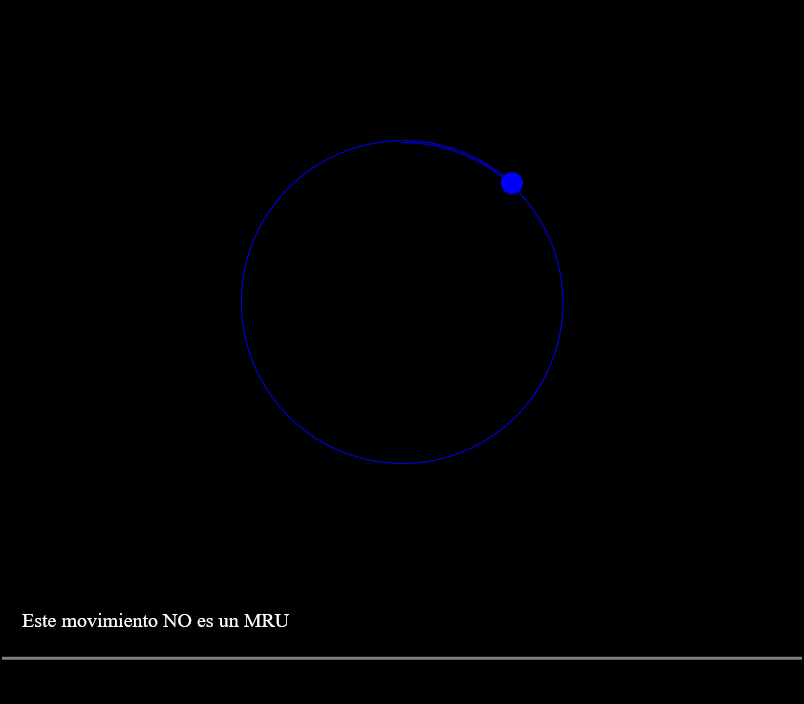
\includegraphics[width=0.9\linewidth]{images/traj1_dt_001.png}
        \caption{$dt=0.01$}
        \label{fig:traj_dt_001}
    \end{subfigure}
    
    \begin{subfigure}{.5\textwidth}
        \centering
        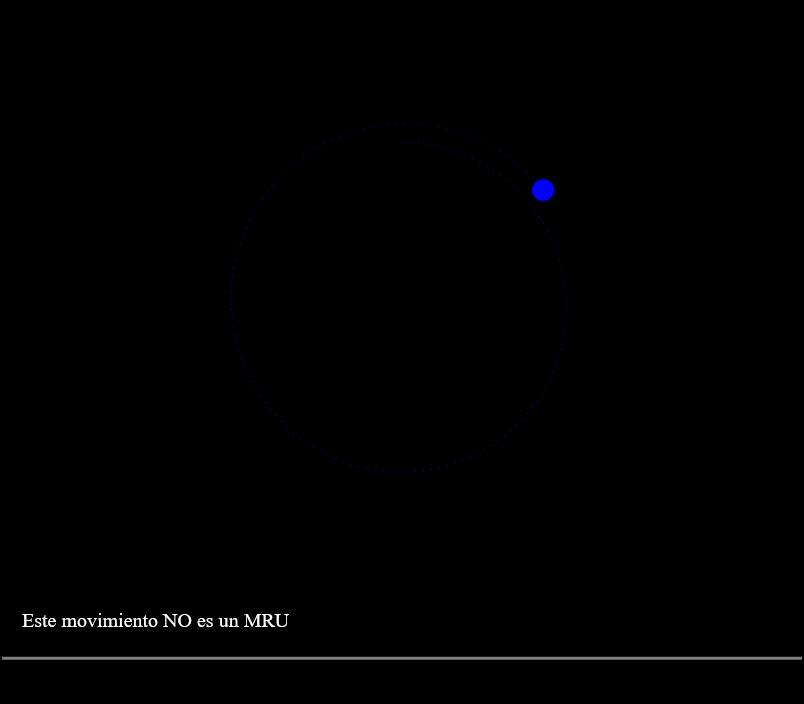
\includegraphics[width=0.9\linewidth]{images/traj1_dt_01.png}
        \caption{$dt=0.1$}
        \label{fig:traj_dt_01}
    \end{subfigure}
    
    \begin{subfigure}{.5\textwidth}
        \centering
        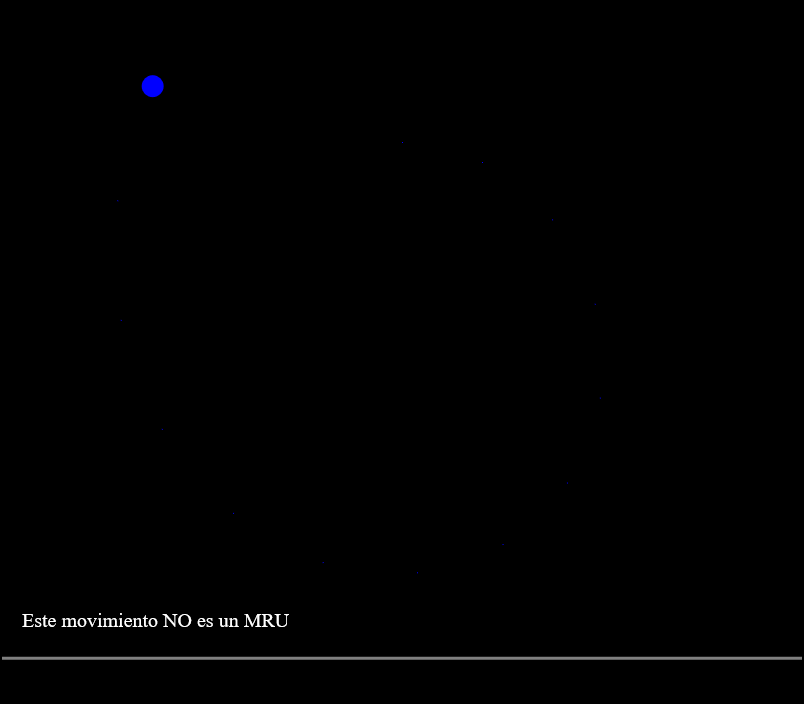
\includegraphics[width=0.9\linewidth]{images/traj1_dt_1.png}
        \caption{$dt=1$}
        \label{fig:traj_dt_1}
    \end{subfigure}
    
\end{figure}
\end{comment}

% Trayectorias de las simulaciones
\begin{figure}[H]
    \centering
    \captionsetup{justification=centering,margin=2cm}
    \subfigure[]{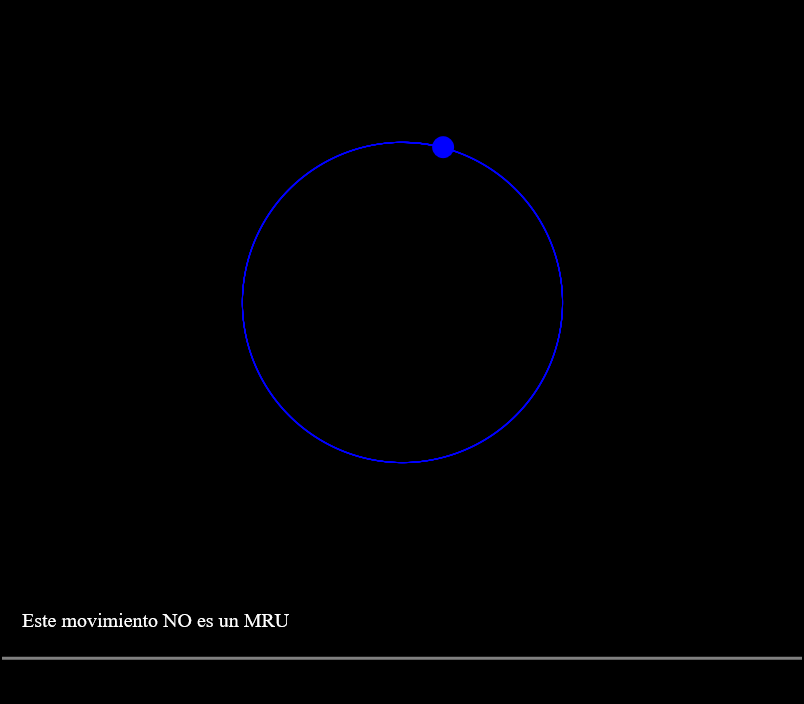
\includegraphics[width=0.45\textwidth]{images/traj1_dt_0001.png}}
    \subfigure[]{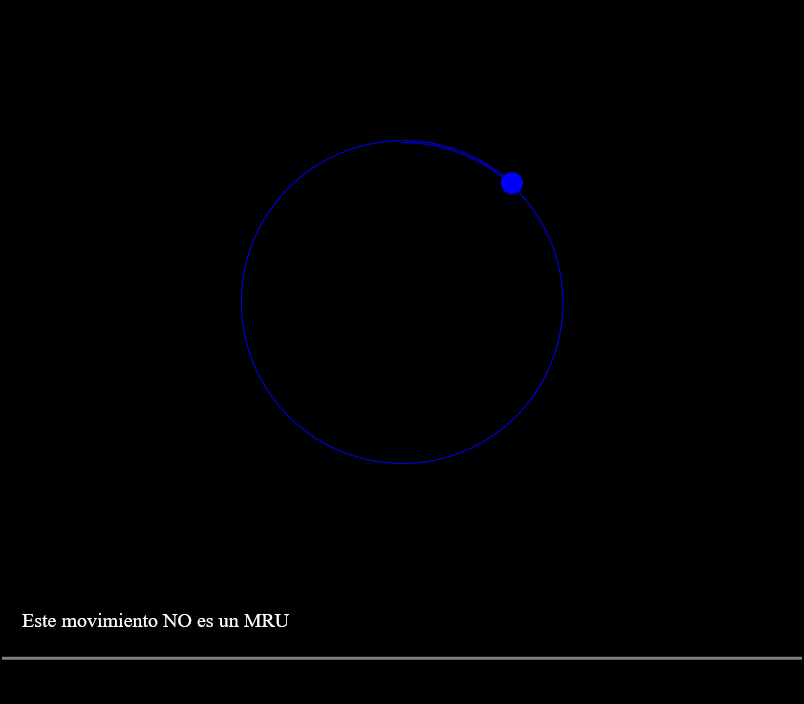
\includegraphics[width=0.45\textwidth]{images/traj1_dt_001.png}} 
    \subfigure[]{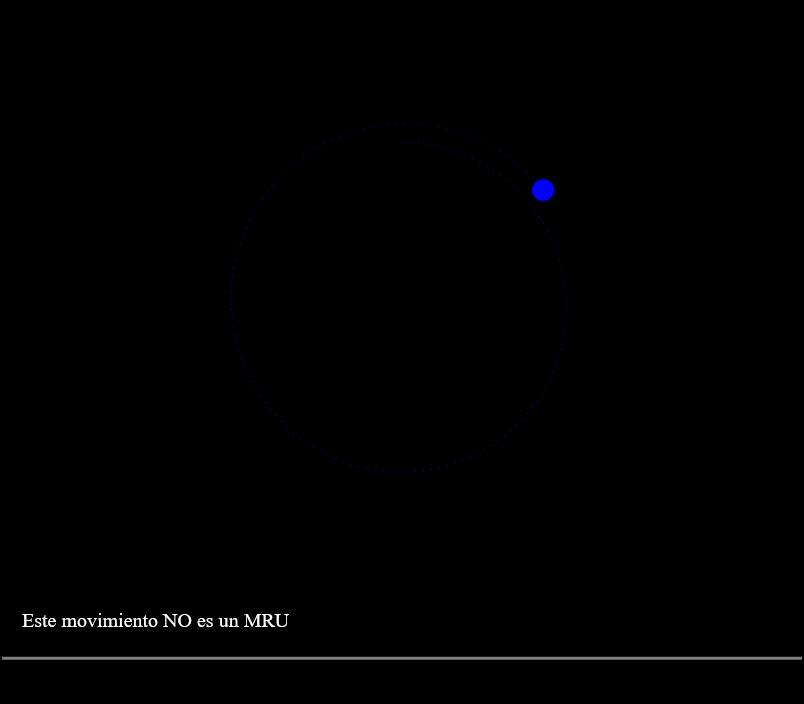
\includegraphics[width=0.45\textwidth]{images/traj1_dt_01.png}}
    \subfigure[]{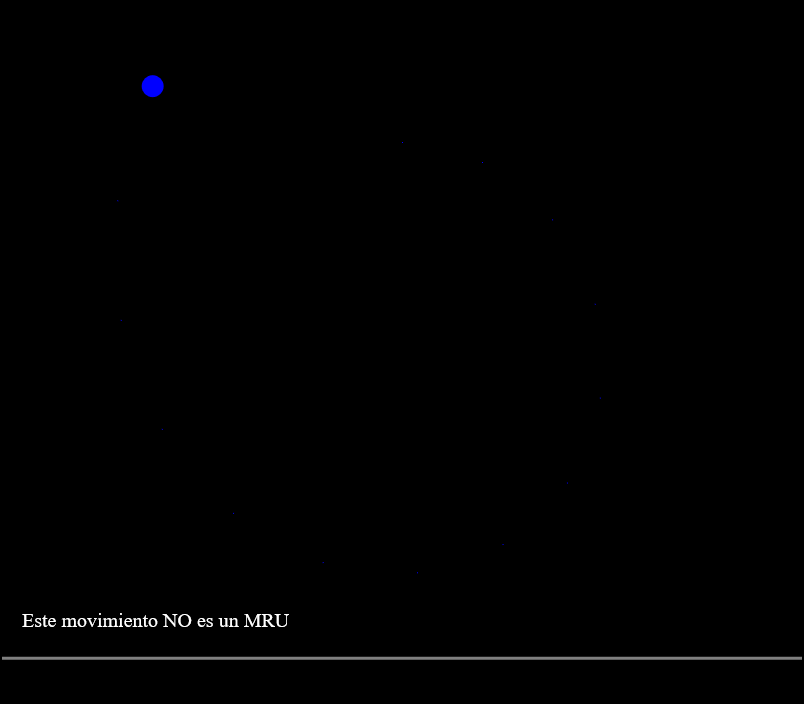
\includegraphics[width=0.45\textwidth]{images/traj1_dt_1.png}}
    \caption{Visualización de las simulaciones \\(a) $dt=0.001$ \, (b) $dt=0.01$ \, (c) $dt=0.1$ \, (d) $dt=1$}
    \label{fig:traj-part1}
\end{figure}

\newpage
Al cambiar la variable de $dt$ en el código de la simulación, se puede observar a primera vista la diferencia del paso temporal de la simulación y la diferencia de la partícula cuando realiza su movimiento. Y tras completar una vuelta se puede observar la desviación de la partícula con respecto a la trayectoria “circular” que se supone que debería estar realizando.

A un valor de $dt$ más pequeño, la simulación se realiza más lento pero con mayor precisión. Se puede observar que realiza más cálculos y la trayectoria es en “línea”. 
Al incrementar el valor de $dt$, la simulación se realiza más rápido y con un paso mayor (describiendose en puntos), pero con menos precisión ya que la desviación a la trayectoria circular que se mencionó antes es mayor, teniendo forma de un espiral. 

Todo esto observado sucede debido a que la variable $dt$ determina la variación temporal de la simulación. Utilizando el módulo Simple Gui, se define esto cuando se crea el timer para la simulación en la línea 147 del archivo antes mencionado donde se observa el siguiente código:

\begin{mintedbox}{python}
...
# Crea un timer para la simulación,
timer = simplegui.create_timer(1000*dt,tick)
\end{mintedbox}


En este módulo y en programas de simulación en computación en general, la pantalla se actualizan varias veces dentro de un segundo (FPS, \textit{Frames Per Second}). En este caso observamos que al crear el \texttt{timer}, primero se pasa como parámetro el paso temporal para la actualización del frame \texttt{1000 * dt} y luego la función principal \texttt{tick} (definida en línea 76) para que ejecute al actualizar el programa. Para que el programa tenga un paso temporal “similar” al del mundo real, $dt$ tiene que valer 0.001 ya que $dt$ está cronometrado en milisegundos.


%%%%%%%%%%%%%%%%%%%%%%%%%%%%%%%%%%%
\newpage
\section{Segunda Parte}
\subsection{Movimiento rectilíneo}
Sabiendo que $a_x(t) = -8 - 6t + 3t^2$ es la función de aceleración que queremos simular y visualizar, para obtener las funciones y expresiones correspondientes para velocidad 
 $v_x(t)$ y de posición $x(t)$ es necesario integrar la aceleración dada. 

Para hallar velocidad $v_x(t)$:
\begin{align*}
        v_x(t) &= \int a(t) \\
             &= \int -8 - 6t + 3t^2\\
             &= -tx - 3t^2 + t^3 + C
\end{align*}

Para hallar velocidad $x(t)$:
\begin{align*}
        x(t) &= \int v_x(t) \\
             &= \int -8t - 3t^2 + t^3 + C\\
             &= -4t^2 - t^3 + \frac{t^4}{4} + Ct + D
\end{align*}

Para realizar esta simulación se toman como condiciones iniciales $x=0m$ y $v_x=0m/s$ para no tener que lidiar con las constantes de integración, de la manera que $C=0$ y $D=0$. Se modifica el archivo \texttt{movimiento.txt} con el fin de estudiar este movimiento ya que sólo se necesita simular una sola dimensión (en eje X).

Este es código de la función \texttt{tick} del archivo \texttt{movimiento.txt} luego de ser modificado:


\begin{mintedbox}{python}
...
# Aqui tenemos las instrucciones que se ejecutan en cada
# paso de la simulación
def tick():
    global time #si uno quiere modificar el valor de una variable global, debe incluir estas líneas.
    global posx
    global velx
    global ax
    
    time += dt #al valor de tiempo previo le suma "dt"
     
    # Actualización de la posición (aquí tenemos el cálculo
    # de la nueva posición basado en el valor previo de 
    # posición y en la forma en la que se está moviendo 
    # el objeto)
    posx = -4*time*2 - time*3+ pow(time, 4)/4
    # Actualización de la velocidad 
    velx = -8*time - 3*time*2 + time*3
    # Actualización de la aceleración
    ax = -6*time + 3*time**2 - 8
    
    # Imprime en pantalla los valores de las variables mencionadas.
    print time,posx
\end{mintedbox}
\textit{Es más conveniente la utilización de pow(var, x) en vez de var**x para las potencias ya que facilita lectura}.

\vspace{0.5cm}
Se corre el programa con valores de $dt=0.01, 0.1, 0.5$ en el intervalo $[0s, 10s]$ obteniendo los siguientes gráficos de posición(x) en función del tiempo(s):

\begin{figure}[H]
    \centering
    \captionsetup{justification=centering}
    \subfigure[]{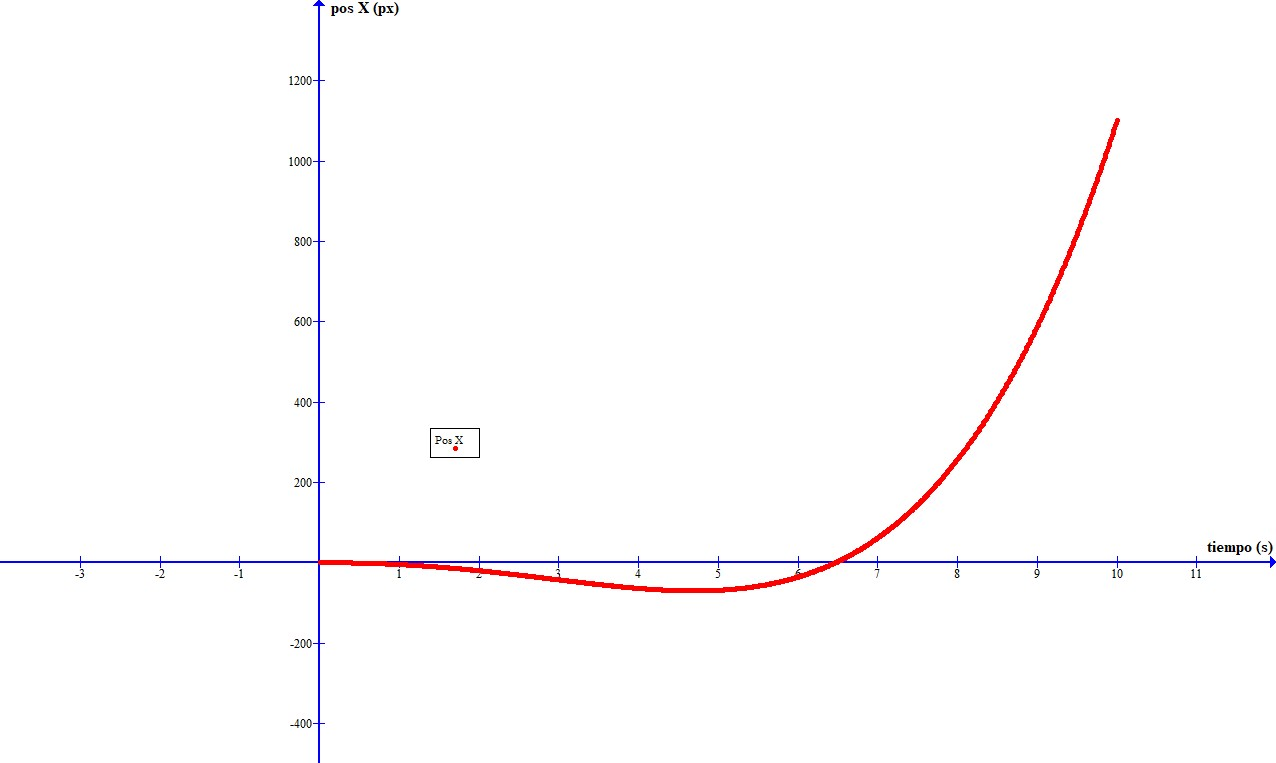
\includegraphics[width=0.5\linewidth]{images/img_graphs/a/traj2a_dt_001.jpeg}}\hfill
    \subfigure[]{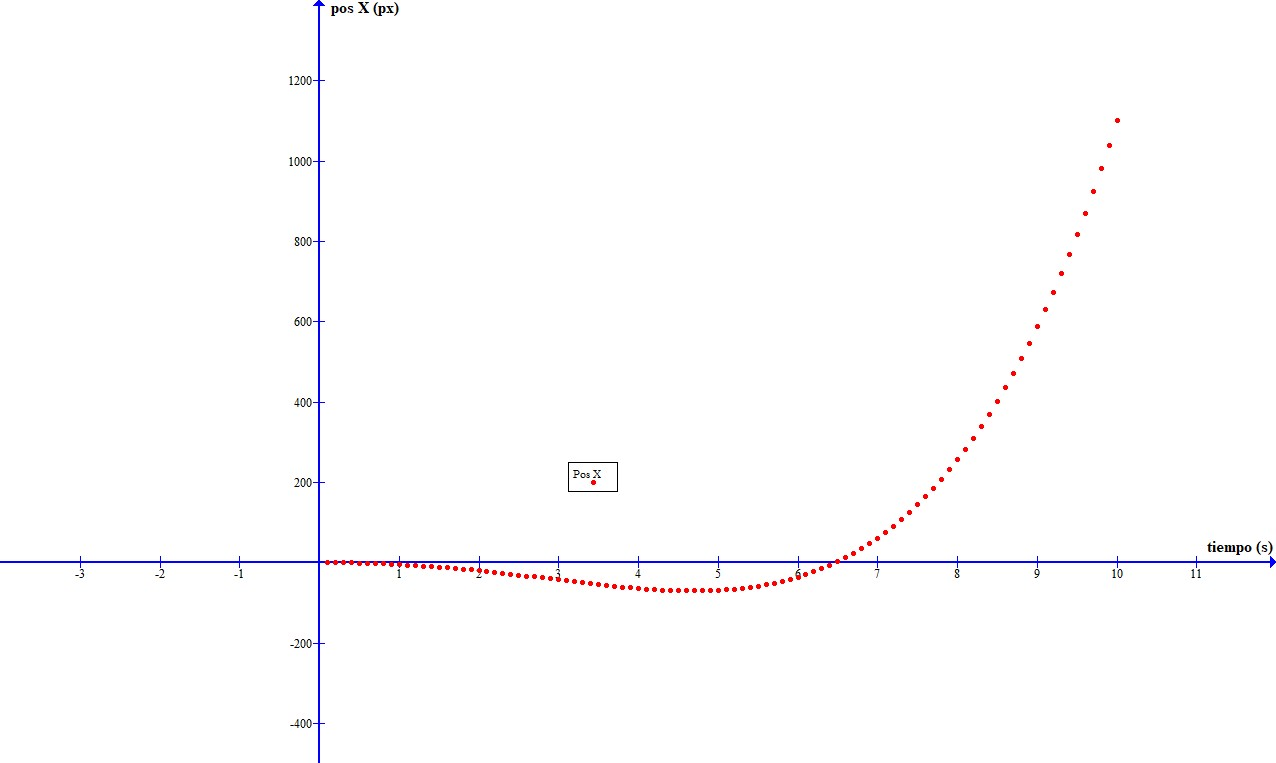
\includegraphics[width=0.5\linewidth]{images/img_graphs/a/traj2a_dt_01.jpg}}
    \subfigure[]{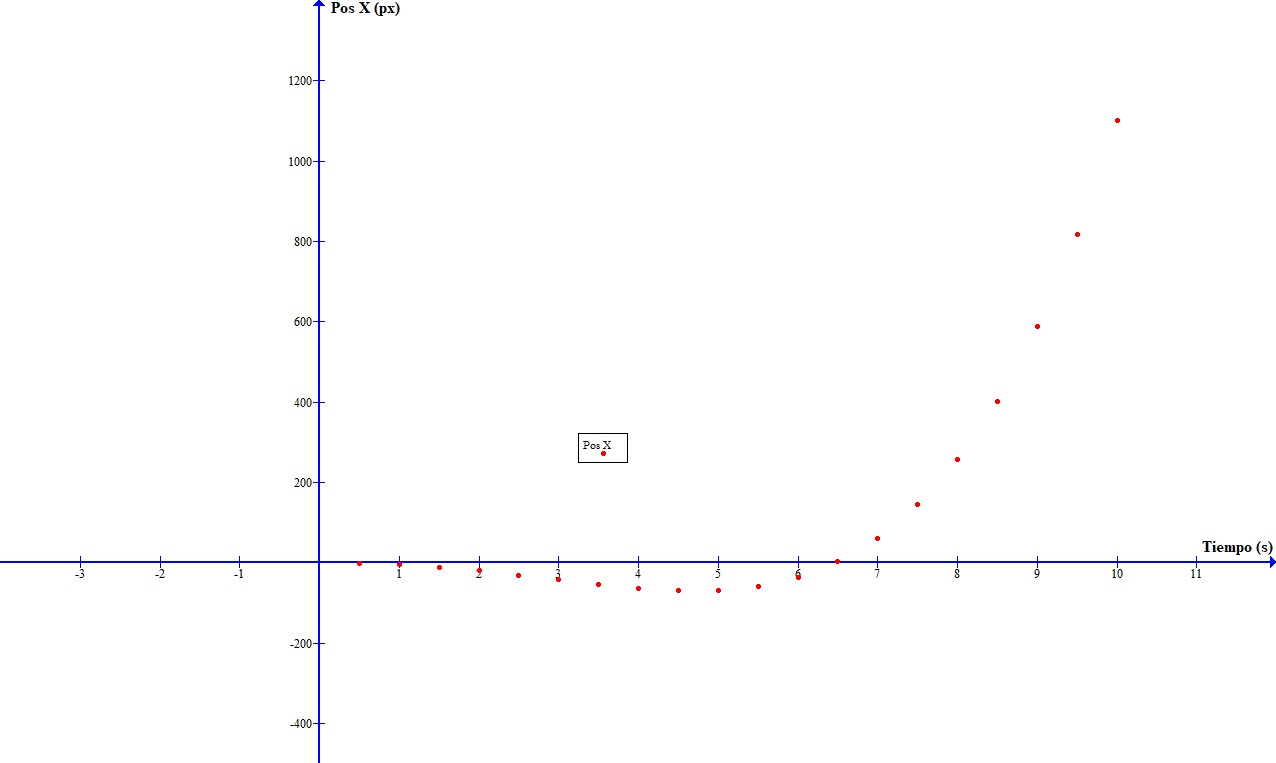
\includegraphics[width=0.5\linewidth]{images/img_graphs/a/traj2a_dt_05.jpg}}
    \caption{Gráficos de posición en eje X (píxeles) en función del tiempo (segundos) en intervalo $[0s, 10s]$\\ (a) $dt=0.01$ \, (b) $dt=0.1$ \, (c) $dt=0.5$}
    \label{fig:part2a}
\end{figure}

En este caso, se hizo una simulación en el eje horizontal (movimiento rectilíneo en eje x). Se puede observar en Figura \ref{fig:part2a} que al aumentar el valor de $dt$, hay más espacio entre los puntos. Esto se debe a que se realiza menos cálculos y se debe a la alargue de la actualización de la pantalla como se mencionó en el análisis de la Primera Parte. Sin embargo, a diferencia del anterior, podemos observar que en estos tres gráficos se mantiene el mismo movimiento, es decir que el movimiento no cambia con respecto a la modificación del paso temporal de la simulación. 

%%%%%%%%%%%%%%%%%%%%%%%%%%%%%%
\subsection{Movimiento compuesto}
Para esta parte de análisis se modificó el código de la línea 89 del archivo archivo \texttt{movimiento\_2d.txt}:

\begin{mintedbox}{python}
...
# Cálculo de la aceleración
    ax = -posx*3 + posx*2 + 1.
    ay = 5*(-posy/sqrt(posx*2+posy*2))
\end{mintedbox}

Se obtuvieron los gráficos de las posiciones en función del tiempo para las simulaciones de $dt=0.001$, $dt=0.01$ y $dt=0.1$

\begin{figure}[H]
    \centering
    \captionsetup{justification=centering}
    \subfigure[]{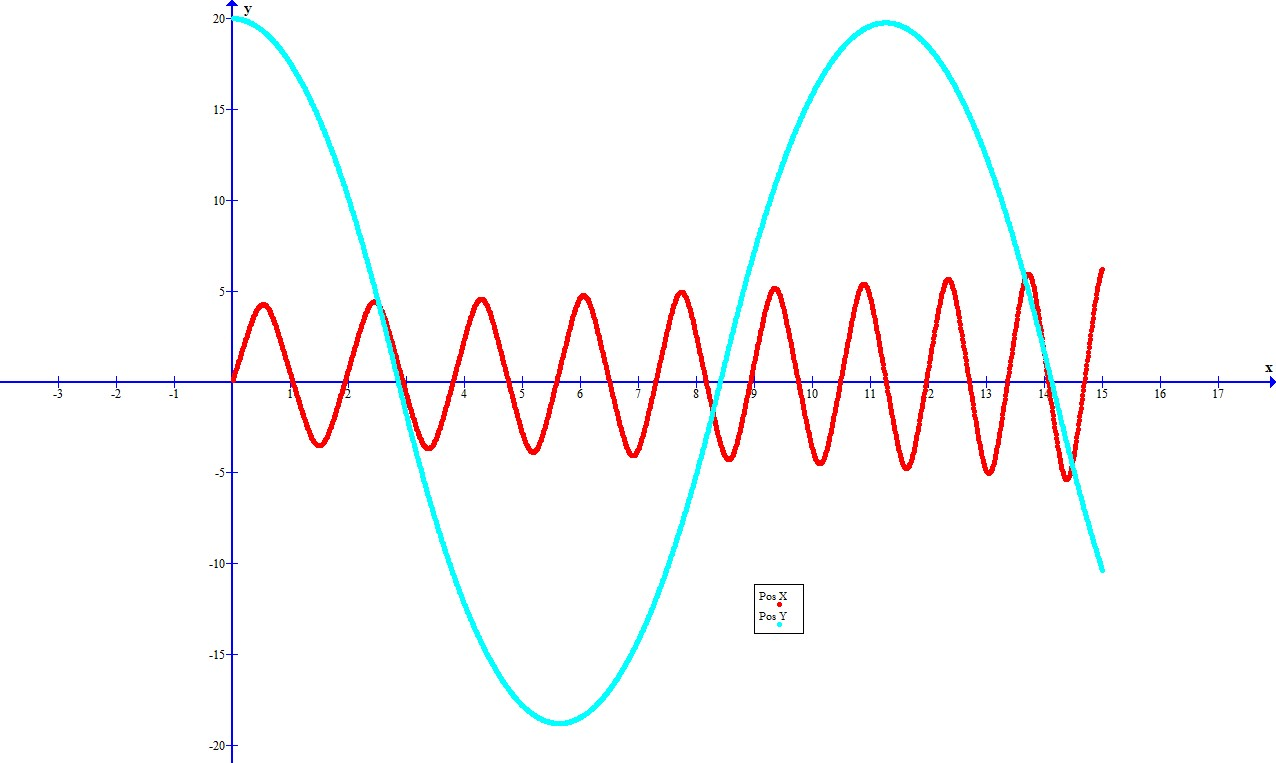
\includegraphics[width=0.5\linewidth]{images/img_graphs/b/traj2_dt_0001.jpg}}\hfill
    \subfigure[]{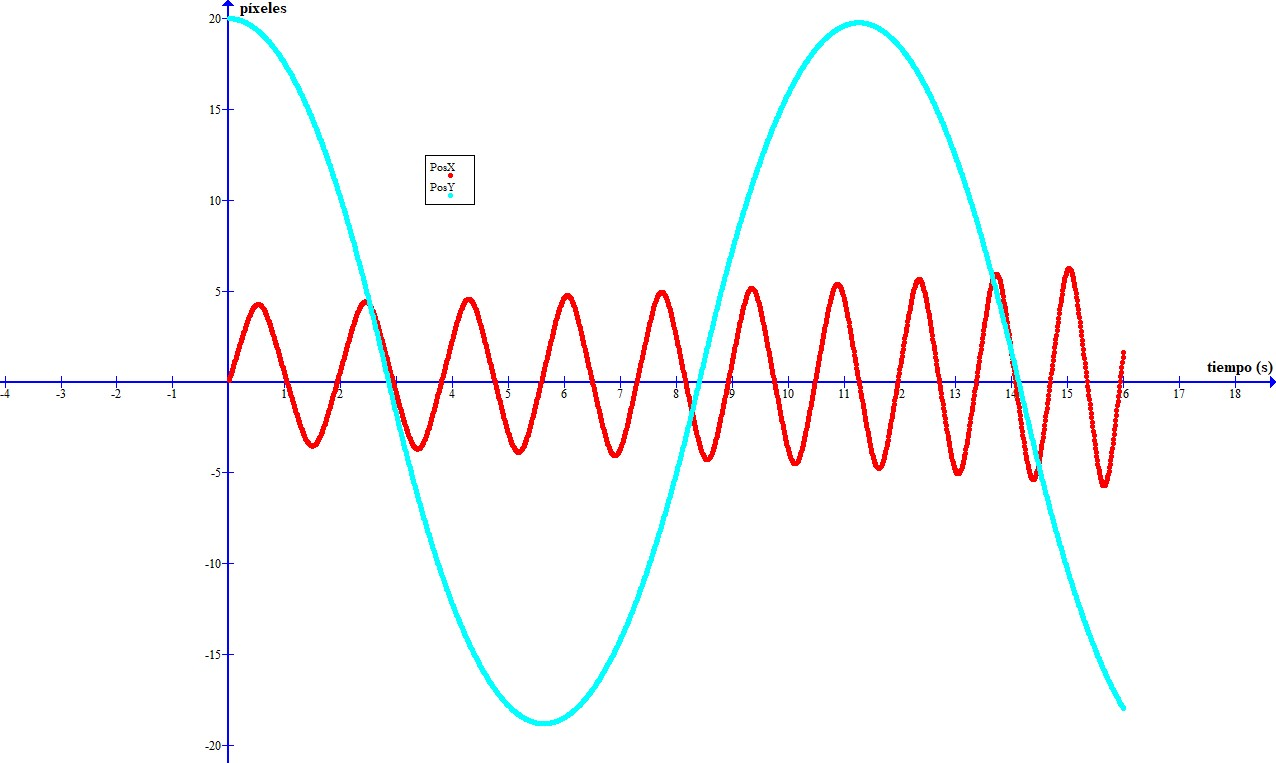
\includegraphics[width=0.5\linewidth]{images/img_graphs/b/traj2_dt_001.jpg}}
    \subfigure[]{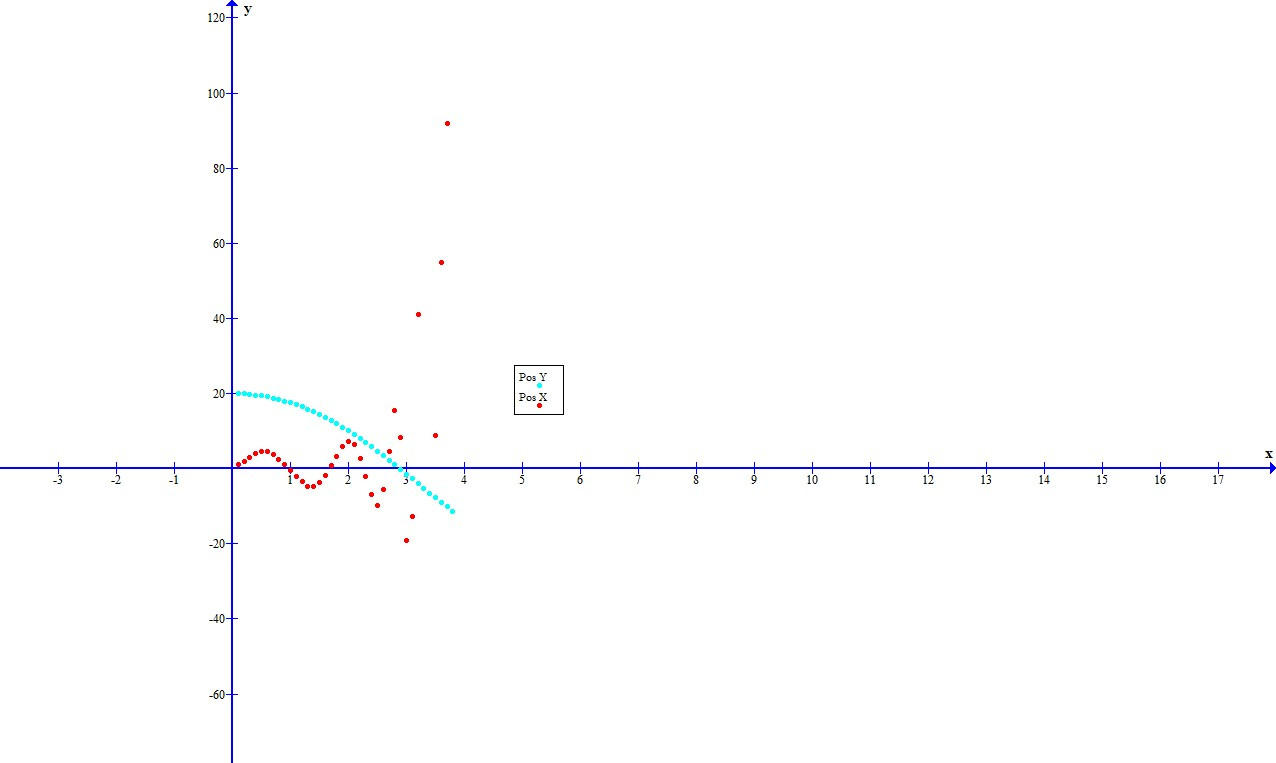
\includegraphics[width=0.5\linewidth]{images/img_graphs/b/traj2_dt_01.jpg}}
    \caption{Gráficos de posición (píxeles) en función del tiempo (segundos) en intervalo $[0s, 15s]$\\ (a) $dt=0.001$ \, (b) $dt=0.01$ \, (c) $dt=0.1$}
    \label{fig:part2b}
\end{figure}

A primera vista podemos tratar el movimiento similar a un movimiento oscilatorio. 


Se puede ver que en los casos de $dt=0.001$ y $dt=0.01$ se diferencian por la cantidad de desplazamiento en un mismo lapso de tiempo. Podemos comparar los gráficos en la parte de la segunda intersección entre posición X (rojo) y la posición Y (celeste) de la partícula en ambos gráficos y observamos que en el caso de $dt=0.01$ tiene un periodo de oscilación más en la posición de eje X (si tratamos el gráfico como una onda). 

En cambio, un caso particular fue el caso de $dt=0.1$ para la misma función introducida para \texttt{ax= -posx **3 + posx **2 + 1}. Donde el programa encuentra un error poco después de los 3 segundos transcurridos de la simulación. Esto sucede debido a que los valores excedieron la capacidad de almacenamiento permitida para los variables del lenguaje del programación, que en este caso es Python 2. Así mismo podemos observarlo visualmente en el gráfico: se puede observar que mientras que en el posición del eje Y mantiene su curso natural, en las posiciones de eje X se dispara a un valor muy grande haciendo detener el programa.

%%%%%%%%%%%%%%%%%%%%%%%%%%%%%%%
\section{Conclusión}
Para ciertos movimientos es posible simular en programas computacionales y para ciertos movimientos no en exactitud. Como se observó en el análisis de este documento, el movimiento simulado puede variar dependiendo del valor del paso temporal asignado para la simulación. Esto sugiere que hay que tener cuidado a la hora de querer simular un movimiento físico dentro de un programa, teniendo en cuenta que pueden surgir este tipo de problema.

Sin embargo, la simulación a su vez es una herramienta  eficaz a la hora de querer estudiar casos de movimientos desconocidos y poder visualizarlas para comprender mejor. También, la utilización y el avance de la tecnología  permite tener una mayor precisión en los cálculos antes que hacerlas manualmente. Es por ello que es importante el aprendizaje del uso de la tecnología para poder aplicarlas a la resolución de nuestros problemas tanto para Física como también en la aplicación de la vida cotidiana. 

\end{document}
